\section{Introdução}

Seja muito bem vindo ao manual do usuário do Grata (Gerenciador de Reuniões e Atas), a ferramenta que irá te ajudar você, caro gerente de projetos, a melhorar suas reuniões.

Este \textit{software} foi desenvolvida para ser uma ferramenta completamente gratuita, com código aberto, e que permite uma custumização das empresas para seus problemas especifícos. Tudo relacionado podem ser encontrados nos seguintes links: \href{https://github.com/FGAProjects/TCC}{TCC}, \href{https://github.com/MrVictor42/Grata-Backend-v2}{Backend}, e \href{https://github.com/MrVictor42/Grata-Frontend-v2}{Frontend}. 

\textbf{Em caso de qualquer dúvida, pertinentes a este projeto, por favor entrar em contato com o desenvolvedor deste projeto pelo email: mrvictor042@gmail.com.}

\textbf{A ferramenta foi desenvolvida para ser gratuita e adaptável as necessidades das empresas, e a custumização de novas funcionalidades, servidores, banco de dados e qualquer coisa além do desenvolvido neste projeto, ficará a cargo da empresa.}

\section{Instalação}

O Grata é uma ferramenta online, não necessitando de instalação, contudo para que seja realizada alterações no mesmo deve ser realizado via código. Pedimos que qualquer desejo de mudança na ferramenta, seja realizada a partir de um \textit{"fork"} nos repositórios do \textit{Github}, linkados acima.

Para ajudar no desenvolvimento de novas funcionalidades, ou ainda alterações no formato original do Grata, todos os códigos relacionados a ferramenta foram implementados utilizando o \textit{Docker}. A seguir, como instalar e utilizar o \textit{Docker} do projeto:

\subsection{Windows}

\subsubsection{Docker}

Para instalar o \textit{Docker} no sistema operacional \textit{Windows}, basta seguir os passos do link a seguir: \href{https://docs.docker.com/docker-for-windows/install/}{Docker-Windows}.

\subsection{Ubuntu}

\subsubsection{Docker}

Para instalar o \textit{Docker} no sistema operacional \textit{Ubuntu} e suas derivações, basta seguir os passos do link a seguir: \href{https://www.digitalocean.com/community/tutorials/how-to-install-and-use-docker-on-ubuntu-20-04}{Docker-Ubuntu}.

\subsubsection{Docker-Compose}

Para instalar o \textit{Docker-Compose} no sistema operacional \textit{Ubuntu} e suas derivações, basta seguir os passos do link a seguir: \href{https://www.digitalocean.com/community/tutorials/how-to-install-and-use-docker-compose-on-ubuntu-20-04-pt}{Docker-Compose-Ubuntu}.

No sistema operacional \textit{Ubuntu} e suas derivações, em ambas os projetos (\textit{frontend/backend}), devem ser rodado os seguintes comandos: 
\begin{itemize}
    \item docker-compose build (Para criar a build do projeto);
    \item docker-compose up (Para rodar o projeto).
\end{itemize}

\section{Como Utilizar?}

\subsection{Tela Inicial e Login}

\begin{figure}[H]
    \centering
    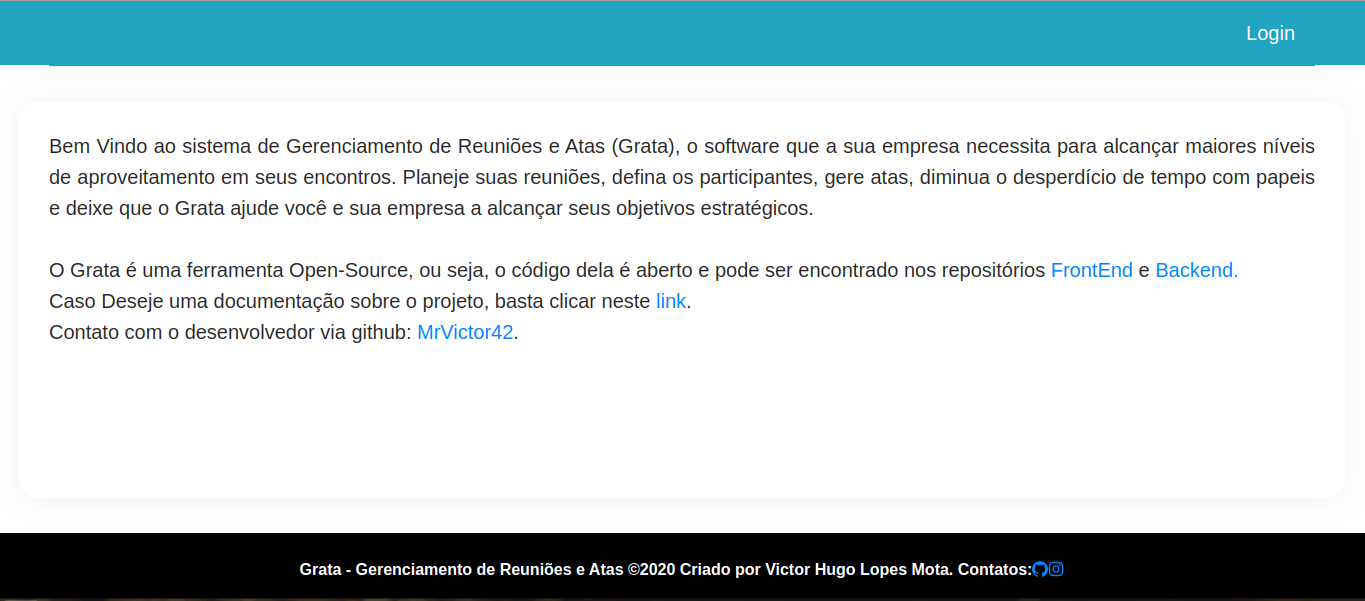
\includegraphics[width=1.0\textwidth]{figuras/tela_inicial.png}
    \caption{Tela Inicial. Fonte: Própria}
    \label{img:tela_inicial}
\end{figure}

A imagem \ref{img:tela_inicial}, mostra a tela inicial da ferramenta, com uma rápida explicação sobre o que é o \textit{software} em questão. Para começar a acessar os recursos da ferramenta, basta clicar em "\textit{Login}".

\begin{figure}[H]
    \centering
    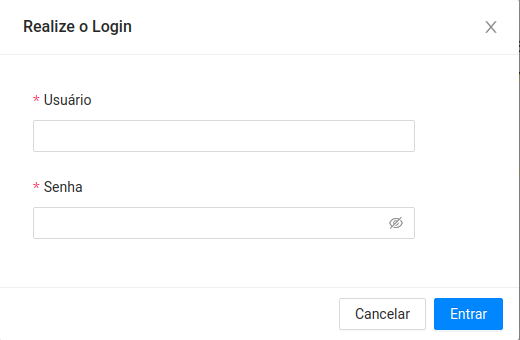
\includegraphics[width=1.0\textwidth]{figuras/tela_login.png}
    \caption{Login. Fonte: Própria}
    \label{img:tela_login}
\end{figure}

Inserindo suas credenciais na ferramenta, você poderá acessar adequeadamente as funções do sistema.

\textbf{No primeiro acesso na ferramenta, entre em contato com o desenvolvedor.}

\subsection{Perfis de Usuários}

Os usuários no Grata são divididos em dois grupos: Administrador e Participante da Reunião.

O \textbf{Administrador}, é aquele que tem as maiores liberdades dentro do sistema, podendo adicionar novos usuários, criar setores, gerencia reuniões, comentar nas reuniões, e é ele que prove os insumos para uma reunião. Este perfil também pode excluir usuários do sistema e alterar as permissões dos demais usuários, ou seja, ele pode transformar um partipante da reunião em um administrador.

O \textbf{Participante}, é aquele que deve ser convidado pelo administrador a compor uma reunião, além de poder comentar sobre a mesma e estar por dentro do que rumo dos projetos em que está participando.

\subsection{Usuários}

\begin{figure}[H]
    \centering
    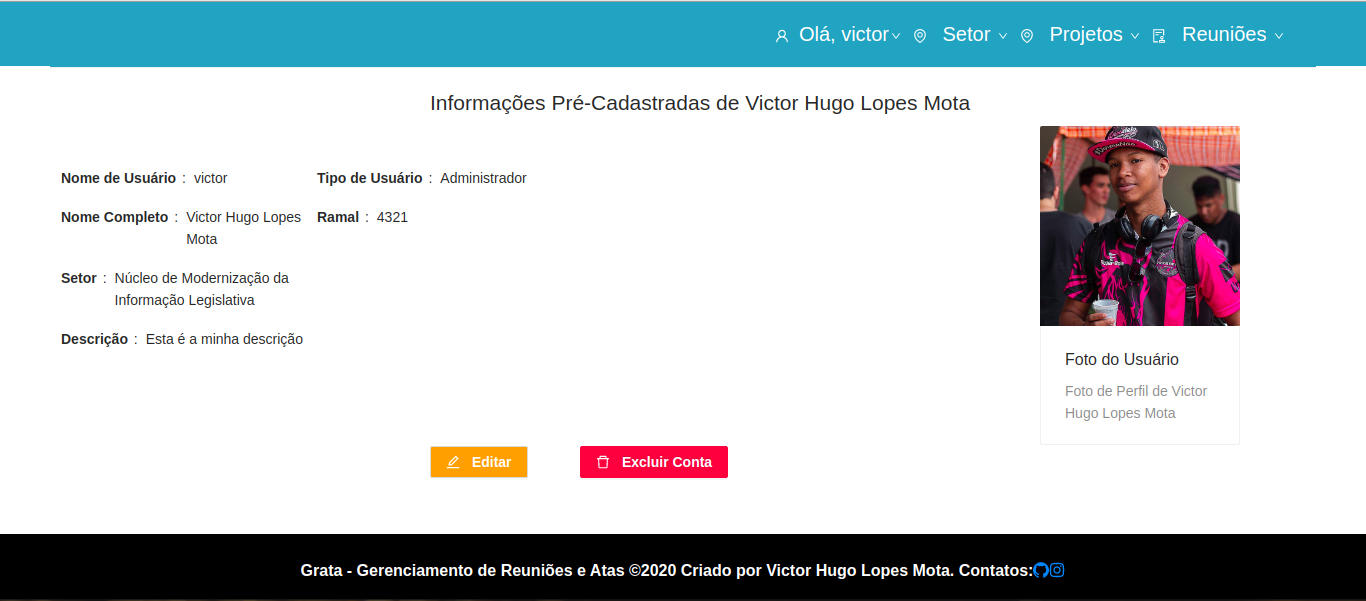
\includegraphics[width=1.0\textwidth]{figuras/tela_perfil.png}
    \caption{Tela de Perfil do Usuário. Fonte: Própria}
    \label{img:tela_perfil_usuario}
\end{figure}

A imagem \ref{img:tela_perfil_usuario}, mostra a tela de perfil de usuário qualquer, contendo suas informações básicas. Todos os usuários podem editar suas informações, além de colocar o setor em que trabalham.

Ao clicar no botão "Editar", o sistema irá mostrar a seguinte tela:

\begin{figure}[H]
    \centering
    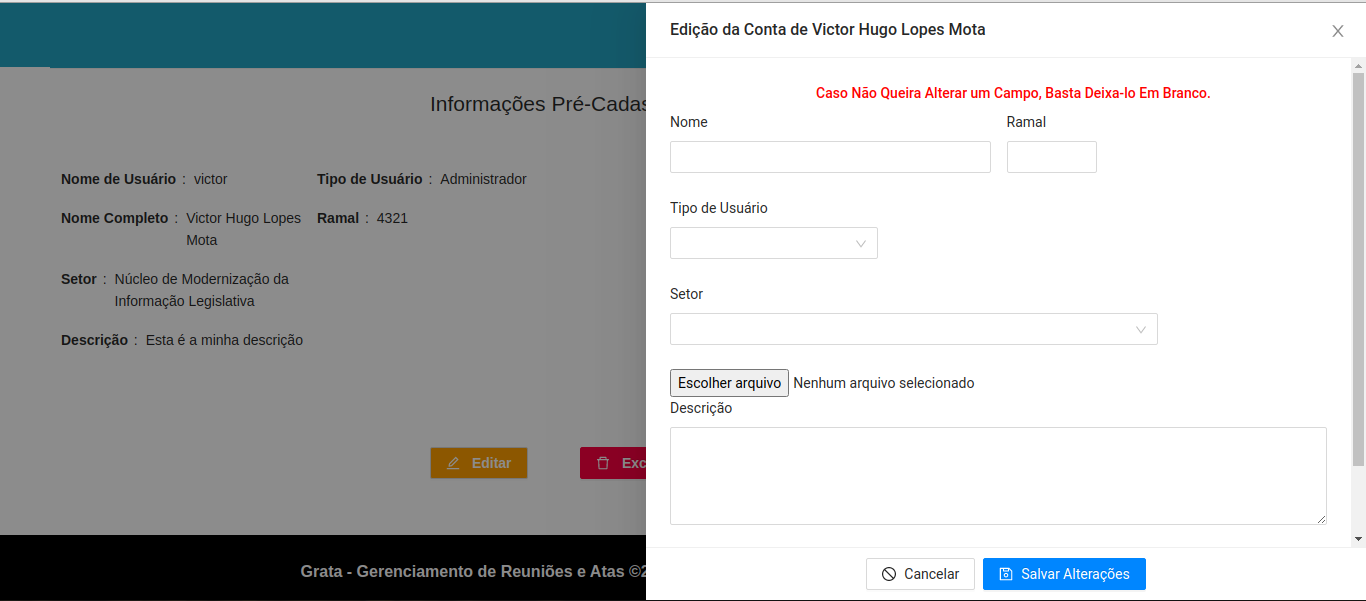
\includegraphics[width=1.0\textwidth]{figuras/edicao_usuario.png}
    \caption{Tela de Edição do Usuário. Fonte: Própria}
    \label{img:tela_edicao_usuario}
\end{figure}

Na tela da imagem \ref{img:tela_edicao_usuario}, mostra os campos que podem ser alterados pelo usuário (Administrador). Os participantes de usuários a partir do processo de edição, podem alterar informações previamente incluidas pelo administrador.

\subsection{Lista de Usuários}

\begin{figure}[H]
    \centering
    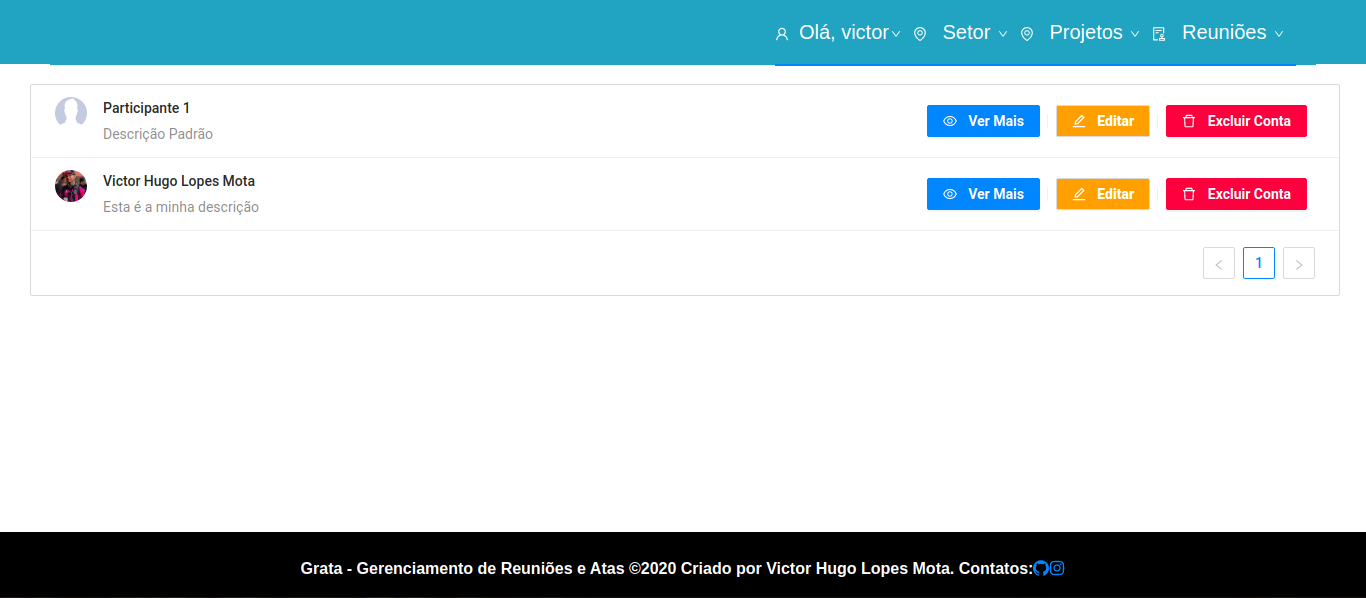
\includegraphics[width=1.0\textwidth]{figuras/lista_de_usuarios.png}
    \caption{Lista de Usuários. Fonte: Própria}
    \label{img:lista_de_usuarios}
\end{figure}

A imagem \ref{img:lista_de_usuarios}, mostra os usuários cadastrados no sistema, mostrando as informações básicas sobre os mesmos. Ao clicar no botão "Ver Mais", é possível visualizar os projetos em que eles estão trabalhando e as reuniões que estão participando. Isso é mostrado na imagem \ref{img:ver_mais}:

\begin{figure}[H]
    \centering
    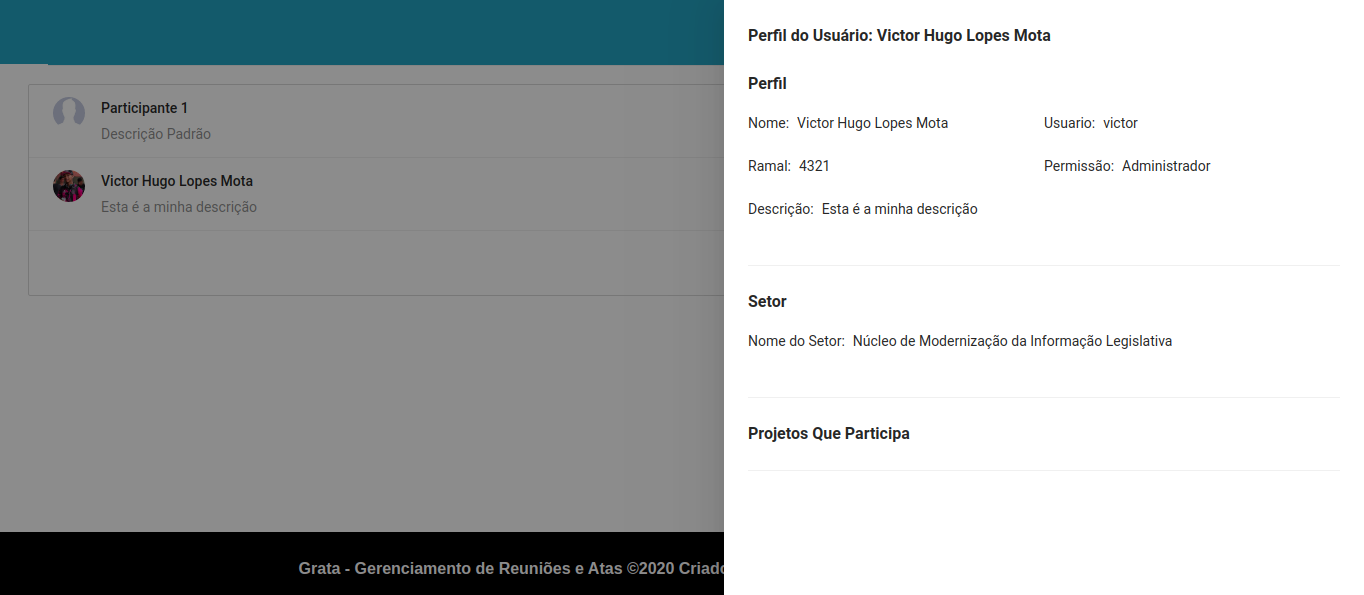
\includegraphics[width=1.0\textwidth]{figuras/ver_mais_usuarios.png}
    \caption{Ver Mais Usuários. Fonte: Própria}
    \label{img:ver_mais}
\end{figure}

\subsection{Navbar}

A \textit{Navbar} do projeto é diferente para os tipos de usuários, mas em todos os casos, ao passar o \textit{mouse} sobre um item da \textit{Navbar}, uma pequena lista de itens irá aparecer e será clicável.

\subsection{Lista de Setores}

\begin{figure}[H]
    \centering
    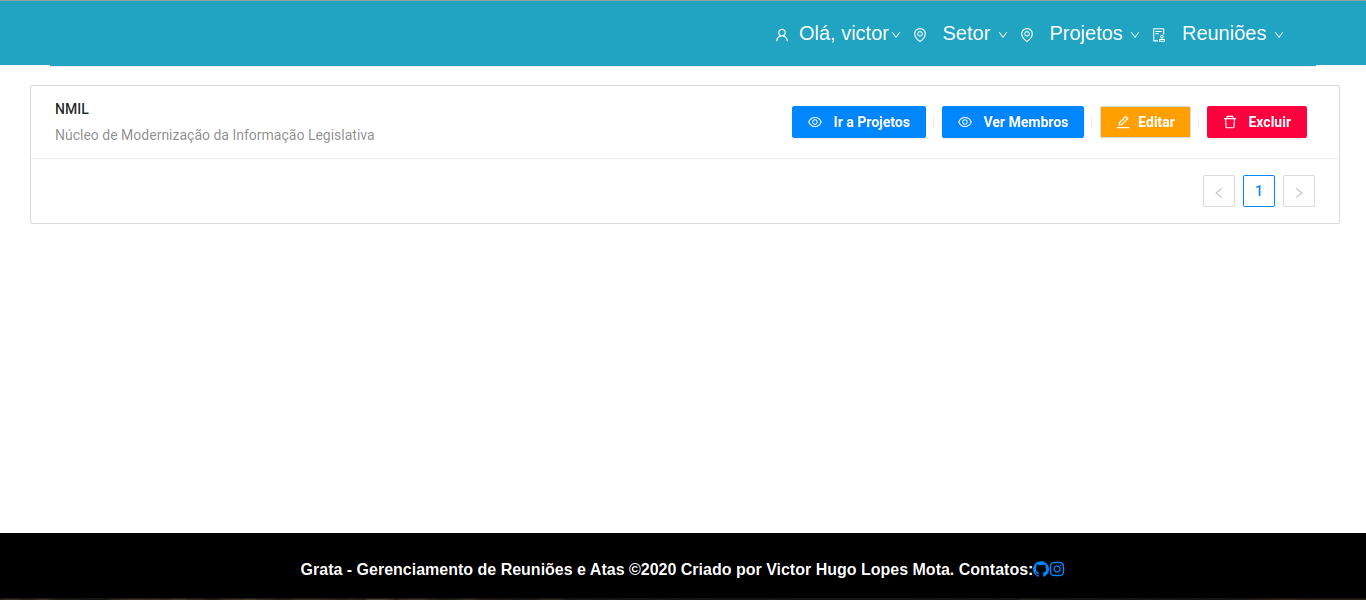
\includegraphics[width=1.0\textwidth]{figuras/lista_de_setores.png}
    \caption{Lista de Setores. Fonte: Própria}
    \label{img:lista_de_setores}
\end{figure}

A lista de setores podem ser vistas por todos os usuários registrados no projeto. Nesta lista, é possível visualizar os projetos e os membros do setor, como mostrado na imagem \ref{img:ver_membros_setores}:

\begin{figure}[H]
    \centering
    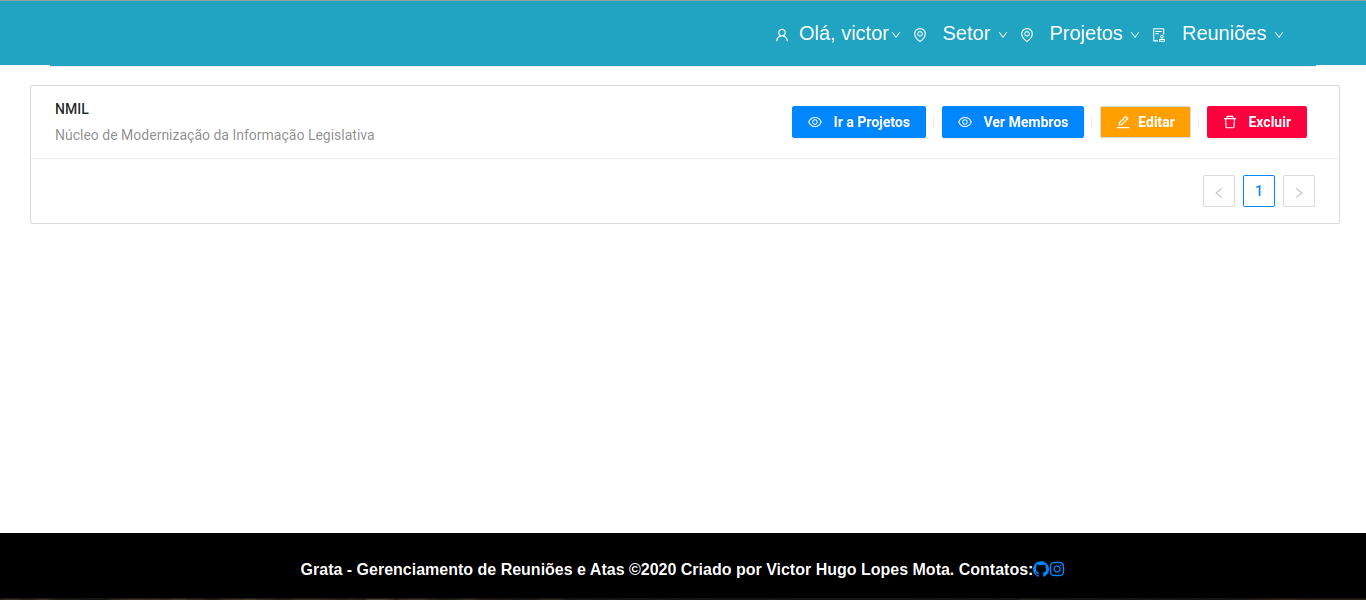
\includegraphics[width=1.0\textwidth]{figuras/lista_de_setores.png}
    \caption{Ver Membros do Setor. Fonte: Própria}
    \label{img:ver_membros_setores}
\end{figure}